\documentclass[10pt]{article}

%\usepackage{hyperref}
\usepackage{alltt}
\usepackage{natbib}
\usepackage{graphicx}
\usepackage{url}
\usepackage{fancyhdr}
\pagestyle{fancy}
\usepackage{trust}
\usepackage{subfigure}
\usepackage{ifthen}

\usepackage{tikz}
\usetikzlibrary{arrows,shadows}
\usepackage[underline=false]{pgf-umlsd}

\lhead{}
\rhead{}
\lfoot{\copyright The University of Kansas, 2013}
\cfoot{\thepage}


\newboolean{submission}  %%set to true for the submission version
\setboolean{submission}{false}
%\setboolean{submission}{true}
\ifthenelse
{\boolean{submission}}
{ \newcommand{\todo}[1]{ } } % hide todo
{ \newcommand{\todo}[1]{ % show todo
   \marginpar{\raggedright\footnotesize{#1}}
               }}
\newcommand{\squash}{\parskip=0pt\itemsep=0pt}

\parskip=\medskipamount
\parindent=0pt


\bibliographystyle{abbrvnat}

\title{ArmoredSoftware Architecture}
\author{Perry Alexander \and Andy Gill \and Prasad Kuklarni \and Leon
  Searl \\
Information and Telecommunication Technology Center \\
The University of Kansas \\
\url{{palexand,andygill,prasadk,lsearl}@ku.edu}}

\begin{document}

\maketitle
\tableofcontents
\listoffigures
\listoftables

\begin{abstract}
  This document describes the evolving ArmoredSoftware architecture.
\end{abstract}

\section{Introduction}

The objective of \textsc{ArmoredSoftware} is to \emph{provide a portable
trusted computing capsule for applications executing in the cloud}.
This capsule, referred to as \emph{armor}, provides three major
functions:

\begin{description}
  \parskip=0pt\itemsep=0pt
\item[Appraisal] -- Request and assess measurement information from
  the operational environment and other armored components.
\item[Measurement] -- Gather run-time measurement information from its
  application
\item[Attestation] -- Assemble and deliver evidence to appraisers in a
  manner that assures measurement integrity
\end{description}

\noindent and is based on concepts from \citet{Coker::Principles-of-R}. 

Figure~\ref{fig:architecture} graphically depicts the major
architectural components of a protected application.  The
\emph{application} is the application to be protected by the
infrastructure.  The \emph{measurement} component performs measurement
operations on the running application while the \emph{attestation}
component gathers measurements and delivers them with cryptographic
assurance of integrity and confidentiality.  The \emph{appraisal}
component requests information from the environment and other
components to assess the overall operational environment.
\emph{Access control} governs access to all critical resources in the
protected application to assure secrets are preserved and enforce
information flow restrictions.

\begin{figure}
  \centering
  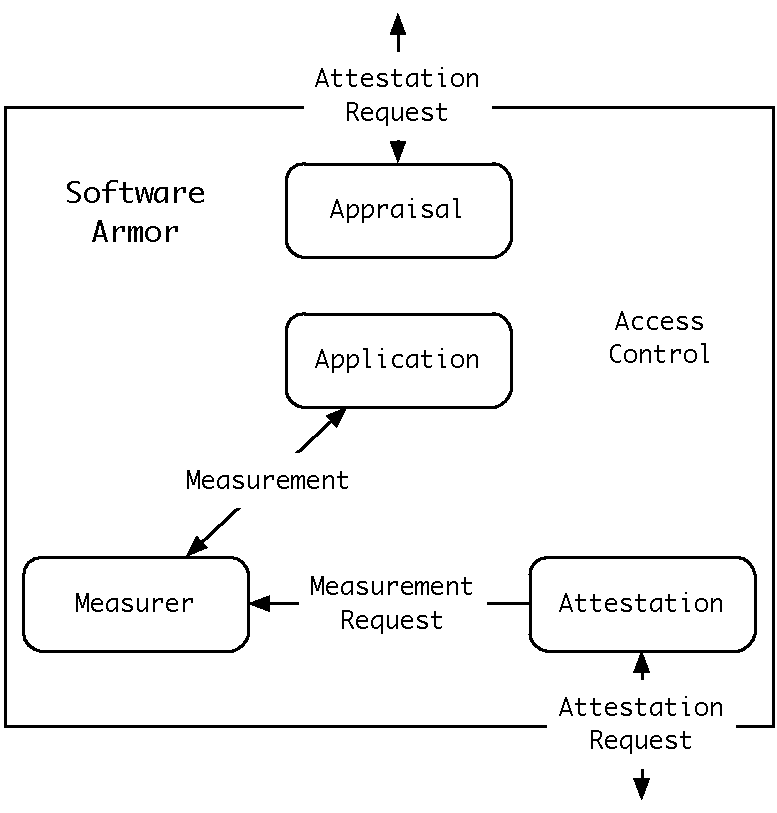
\includegraphics[width=0.5\textwidth]{figures/architecture.pdf}
  \caption{\textsc{ArmoredSoftware} component architecture showing
    major components of the remote attestation process.}
  \label{fig:architecture}
\end{figure}

Figure~\ref{fig:system} graphically represents the interaction among
protected components while Figure~\ref{fig:sequence} shows the
sequencing of interactions during appraisal.  A component's appraisal
module will request information from a second component's attestation
module.  The attestation model will select an attestation protocol
that instructs the measurer what information to gather and in what
sequence.  The measurer executes that protocol that in turn gathers
information from the running process, accesses the module's virtual
TPM (vTPM) and makes appraisal requests of other
\textsc{ArmoredSoftware} instances.  The attestation module assembles
measurement results into a evidence package that is returned to the
requesting appraiser with cryptographic assurances of integrity and
confidentiality as required.  Upon receiving the package, the
appraiser assesses cryptographic signatures and encryption to
determine the trustworthiness of the measurements, then assesses
measurements to determine the trustworthiness of the component being
appraised.\footnote{Note that the same process occurs when appraising
  the component's operational environment with either the appraiser or
  target replaced by operational infrastructure.}

\begin{figure}[hbtp]
  \centering
  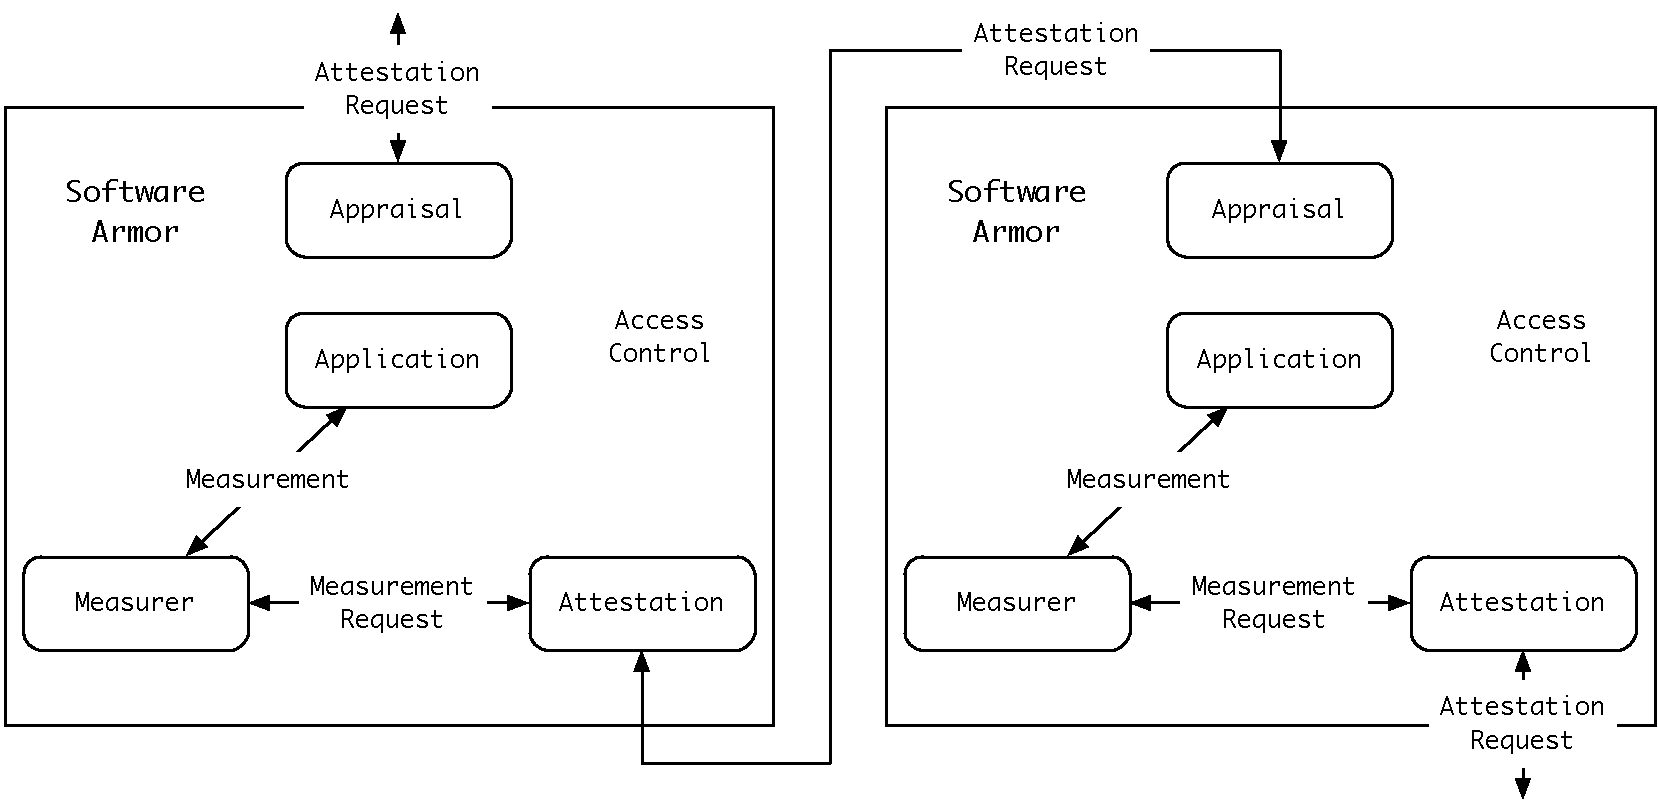
\includegraphics[width=0.5\textwidth]{figures/system.pdf}
  \caption{System Architecture}
  \label{fig:system}
\end{figure}

\begin{figure}
\begin{footnotesize}
  \begin{sequencediagram}
    \newthread[white]{appr}{Appraiser}
    \newinst[2]{attest}{Attestation}
    \newinst[2]{meas}{Measurer}
    \newinst[2]{app}{Application}
    
    \begin{call}{appr}{Attestation Request}{attest}{Attestation}
      \begin{callself}{attest}{Protocol Selection}{Attestation Preparation}
      \begin{call}{attest}{Measurement Requests}{meas}{Measurement Values}
        \begin{call}{meas}{Measurement Calls}{app}{Measurement Values}
        \end{call}
      \end{call}
      \end{callself}
    \end{call}
    \begin{callself}{appr}{Appraisal}{Execute Decision}
    \end{callself}
  \end{sequencediagram}
\end{footnotesize}
\caption{Architecture component interaction}
\label{fig:sequence}
\end{figure}

\section{System Architecture}

\subsection{Measurement}

Figure~\ref{fig:measurement} graphically shows the processing of
requests for measurements by the measurement
component. Figure~\ref{fig:measurement-1} shows how a measurement
request is processed while Figure~\ref{fig:measurement-2} shows how a
response is generated.

The measurement component is a collection of measurement capabilities
for achieving various measurement goals.  Measurement capabilities
will range from simple checks to determine the presence or absence of
resources to sophisticated run-time monitoring capabilities.  It will
be possible to add and remove measurement capabilities from the
measurer at run-time.

Measurement selection chooses and instantiates a measurement
capability for a particular measurement task.  Measurement tasks from
the attestation component are abstract requests for information.
Measurement selection is responsible for instantiating those requests
with specific, executable measurement instances.

Measurement execution causes a measurement capability to execute,
manages execution and returns measurement results.  Execution is more
than simply execution of a program and includes monitoring, exception
handling and any bookkeeping required to prepare and clean up
following execution.

Measurement capabilities may need to access the vTPM for storing
measurement results, accessing stored results, or for generating
cryptographic evidence in support of assessment.  The vTPM will not be
a part of the measurer, but will be shared by all components
comprising the armor.

The measurement subsystem is protected by access control.  It
is responsible for protecting the application and ensuring sensitive
information is not leaked via the measurement process.

\begin{figure}
\centering 
\subfigure[Request processing]{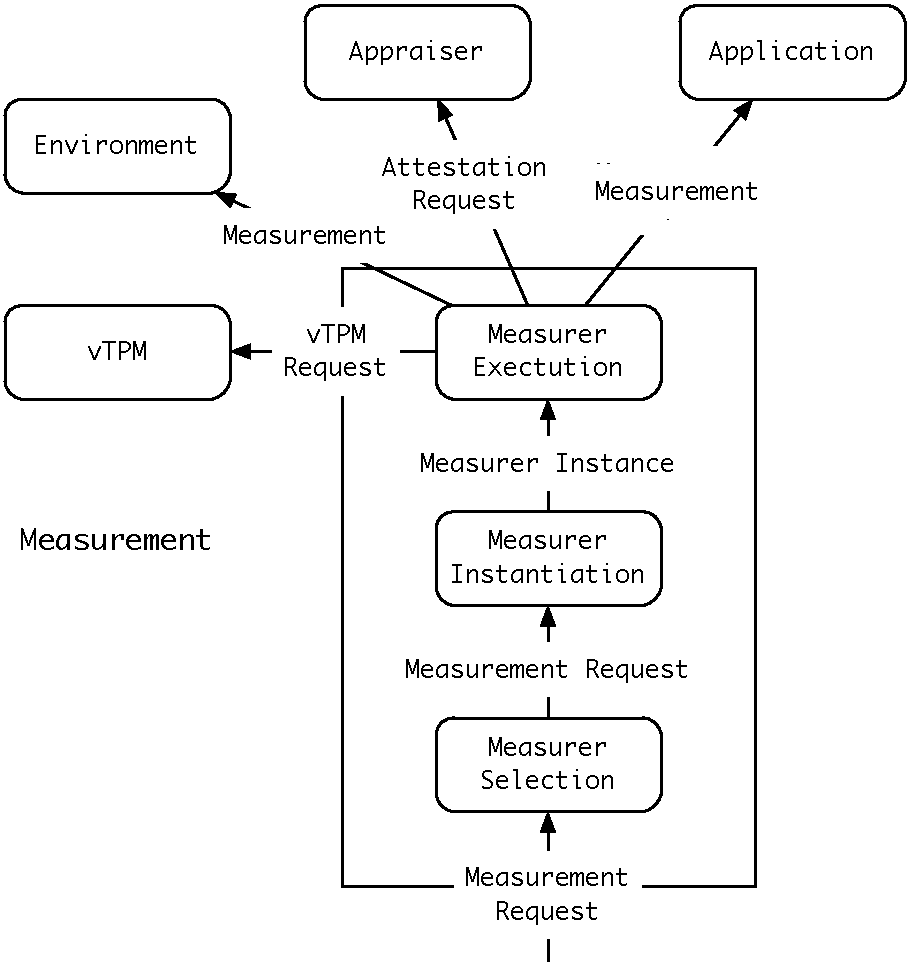
\includegraphics[width=0.450\textwidth]{figures/measurement-1.pdf}\label{fig:measurement-1}}
\subfigure[Response processing]{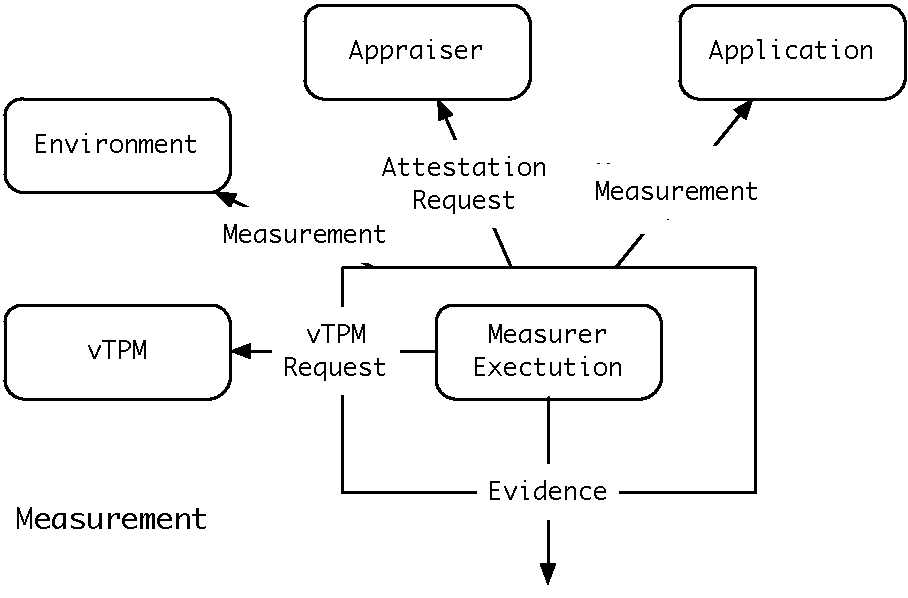
\includegraphics[width=0.450\textwidth]{figures/measurement-2.pdf}\label{fig:measurement-2}}
  \caption{Measurement request processing and response}
  \label{fig:measurement}
\end{figure}

\subsection{Attestation}

Figure~\ref{fig:attestation} graphically shows the processing of an
attestation request by an ArmoredSoftware attestation component.  The
attestation request specifies information requested by an appraiser.
Upon receipt, the \emph{Attestation Protocol Selector} or \emph{AP
  Selector} identifies one or more \emph{Attestation Protocols} that
could satisfy the appraisers request.  The protocol is passed to the
\emph{AP Instantiation} process that selects specific mechanisms for
achieving individual requests in the AP.  The resulting protocol
instance is passed to \emph{AP Execution} where it is executed by: (i)
making requests to the component's vTPM; making requests to another
components attestation service; or (iii) invoking the measurer on the
component's associated application.

\begin{figure}
\centering 
\subfigure[Request processing]{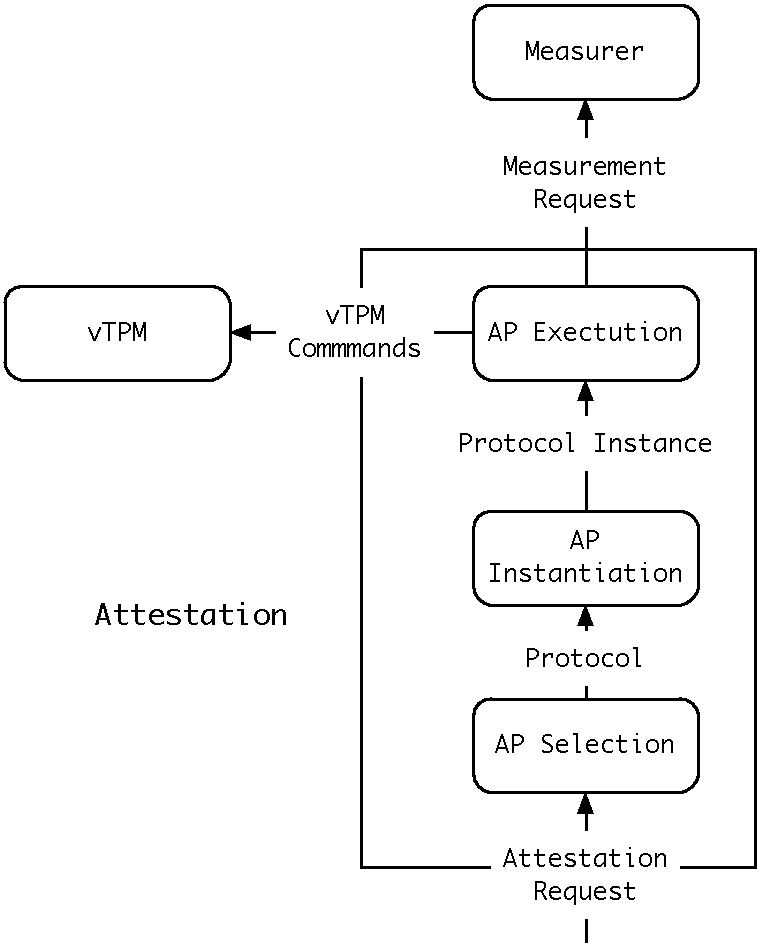
\includegraphics[width=0.450\textwidth]{figures/attestation-1.pdf}}
\subfigure[Response processing]{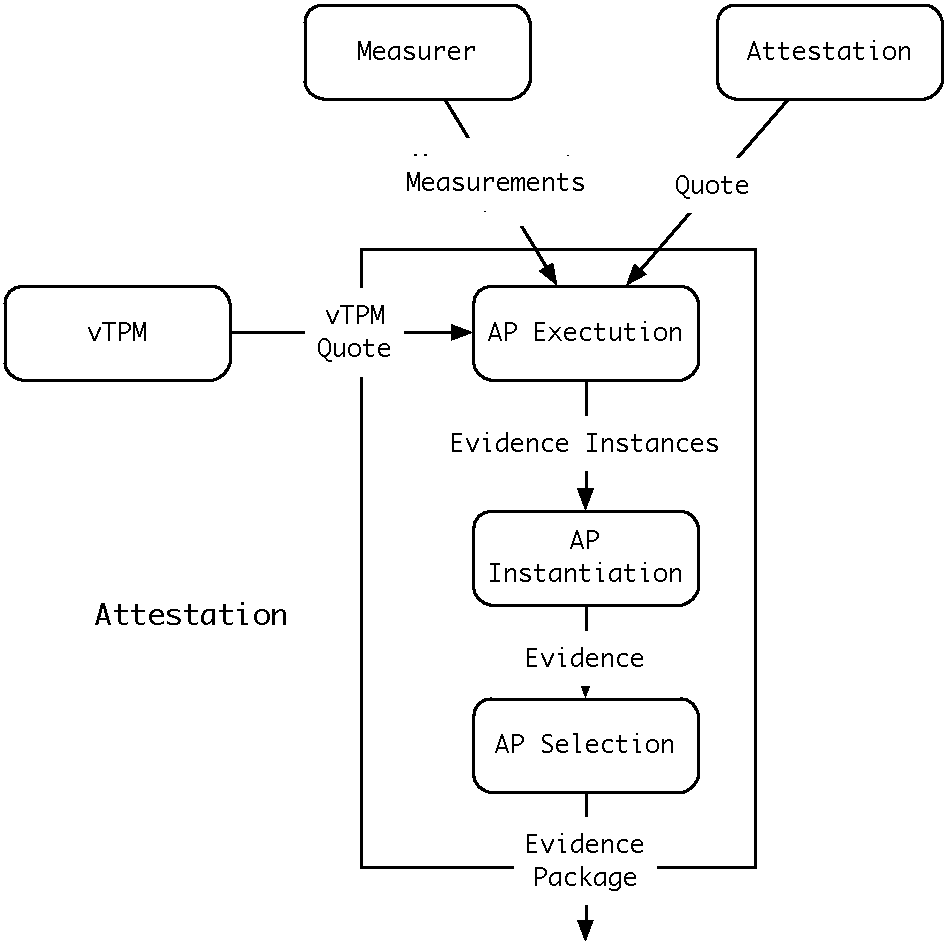
\includegraphics[width=0.450\textwidth]{figures/attestation-2.pdf}}
  \caption{Attestation request processing and response}
  \label{fig:attestation}
\end{figure}

The results of request to the vTPM, another attestation component, and
the local measurer are returned as vTPM quotes, evidence packages, and
measurements respectively.  The AP Execution component monitors
execution and collects various results for processing by the AP
Instantiation component.  AP Instantiation assembles individual
measurement, vTPM and appraisal results into a package representing
information requested in the attestation request.  The AP Selection
component uses cryptographic techniques to provide assurances to the
appraiser requesting information that evidence can be trusted.
Finally, the evidence package is returned to the requesting appraiser
where it is evaluated.

\subsection{Appraisal}

Appraisal assesses the result of an attestation request to determine
if: (i) the evidence received is trustworthy; and (ii) if the
system described by that evidence is trustworthy.  While attestation
is responsible for gathering and delivering measurement information,
appraisal is responsible for assessing it.

\subsection{TPM and vTPM}

Elements of the ArmoredSoftware capsule will share access to a vTPM
associated with the capsule.  That vTPM will be constructed with
root-of-trust in a hardware TPM (hTPM), but must be migratable among
elements of the cloud infrastructure.

\subsection{Access Control}

Access control is omnipresent in the capsule and is responsible for
protecting both the application and elements of the armor.  We
anticipate using a Flask-based MAC style, but may change that approach
as we become more aware of our needs.

\section{Component Interaction}

\subsection{Migration}

\appendix

%%\input{glossary}

%%\nocite{}

\bibliography{architecture}

\end{document}
